\documentclass[11pt]{article}
\usepackage{amsmath, amssymb, amscd, amsthm, amsfonts}
\usepackage{graphicx}
\usepackage{hyperref}
\usepackage[dvipsnames]{xcolor}

\oddsidemargin 0pt
\evensidemargin 0pt
\marginparwidth 40pt
\marginparsep 10pt
\topmargin -20pt
\headsep 10pt
\textheight 8.7in
\textwidth 6.65in
\linespread{1.2}

\title{Course Report: Regression}
\author{Nan He}
\date{}

\newtheorem{theorem}{Theorem}
\newtheorem{lemma}[theorem]{Lemma}
\newtheorem{conjecture}[theorem]{Conjecture}

\newcommand{\rr}{\mathbb{R}}

\newcommand{\al}{\alpha}
\DeclareMathOperator{\conv}{conv}
\DeclareMathOperator{\aff}{aff}

\begin{document}

\maketitle

%\begin{abstract}
%(Abs)
%\end{abstract}

\section{Main objective of the analysis}\label{section-introduction-1}
In this assignment, I will be using one of my own chemical data set.
In chemistry, the interaction of gas molecules with a polarized surface is a interesting topic.
It is especially suitable to be used as a model system to model weak interactions.
I have a data set derived from vibrational spectrum that listed the total energy of carbon monoxide (CO) on a salt (NaCl) surface.
The data entries include 1) the C-O bond length, 2) the distance of CO center to the salt surface, 3) the angle of the CO molecule with the norm of the salt surface. And the label is the total energy at this position.

\begin{figure}[h]
\centerline{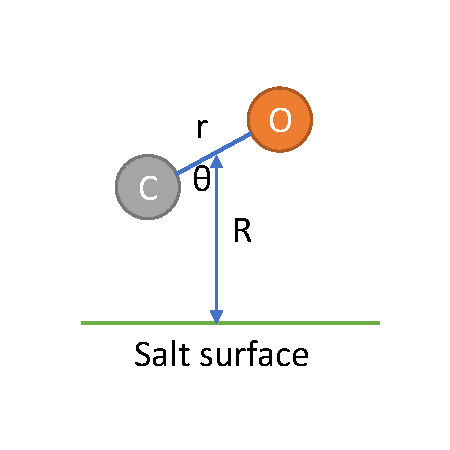
\includegraphics[scale=0.8]{fig1.pdf}}
\caption{An geometrical illustration of the three properties for each data point.}
\end{figure}

\newpage

Example data are:
\begin{figure}[h]
\centerline{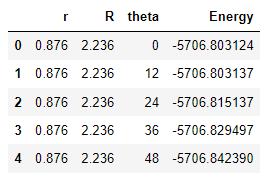
\includegraphics[scale=0.8]{data1.png}}
\caption{The raw data read directly from experiments.}
\end{figure}

The data include the above three parameters, which uniquely defined a location of a CO molecule, and the energy measured at that location.

The objective of this report is to fit those data into a model, so we can predict the CO energy at any position, without conducting new experiments.

\section{Data exploration, cleaning, and feature engineering}\label{section-introduction-2}
The first step is to read raw data (in Excel spreadsheet) into a pandas data frame. This is done using xlrd package.
The next step is to transform the angular parameter theta ($\theta$) into a non-periodic variable.
The simplest solution is to use $cos(\theta)$ instead of $\theta$ as the angular parameter, since $cos(\theta)$ defines a new unique parameter ranging from -1 to 1.
Finally, we will drop all incomplete data (with any of the parameter empty).
The final shape of the data frame is (4608,4).

\begin{figure}[h]
\centerline{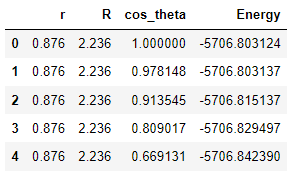
\includegraphics[scale=0.8]{data2.png}}
\caption{The data ready for analysis.}
\end{figure}

\section{Testing different models}\label{section-model}
In this section, I will fit the energy using the three geometrical variables.
I will test three regression models with the same train-test split.
80\% of the data points will be used as training set, and the rest 20\% as test set.
The first model is a simple multi-variable linear regression.
The model is fitted on the training set, the $R^2$ on the training set is 0.177.
Then I use this on the test set, the predicted data (y\_pred) are plotted against the real data (y\_test).
\begin{figure}[h]
\centerline{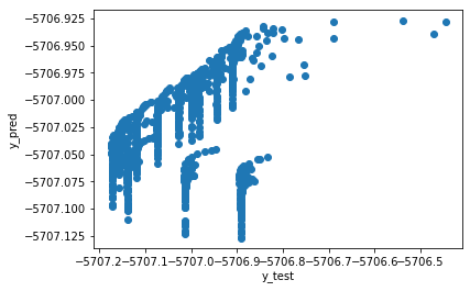
\includegraphics[scale=0.6]{fit1.png}}
\caption{simple linear regression, $R^2=0.142$.}
\end{figure}
The $R^2$ is only 0.142, and the predicted and real data differs significantly, so the simple linear regression is not a suitable model to describe their relationship.

\newpage

The second model is a linear regression with 4th-order polynomial features.
I fit the model on the training set; the $R^2$ is 0.980.
Similarly, I plotted the predicted data (y\_pred) vesus the real data (y\_test).
\begin{figure}[h]
\centerline{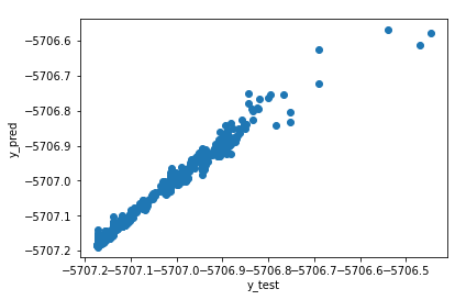
\includegraphics[scale=0.6]{fit2.png}}
\caption{Polynomial regression (4th-order), $R^2=0.981$.}
\end{figure}
The polynomial regression provides a much better results in term of the prediction accuracy on the test set ($R^2=0.981$), and it has similar $R^2$ as in the training set. These results indicate that this 4th-order polynomial regression model captures the general trend of the original data well, without significant over-fitting.

The last model is a linear regression with 4th-order polynomial features, plus an L2 regularization.
The $\alpha$ for the L2 regularization is 1.0.
The $R^2$ on the training set is 0.843.
The scatter plot for predicted data (y\_pred) vesus the real data (y\_test) is:
\begin{figure}[h]
\centerline{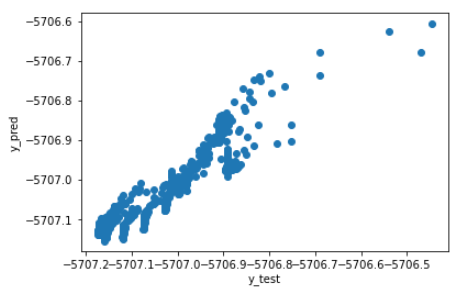
\includegraphics[scale=0.6]{fit3.png}}
\caption{Polynomial regression (4th-order), $R^2=0.838$.}
\end{figure}

The $R^2$ on the test set is 0.838, similar with that on the training set.
The regularization decreases the prediction accuracy comparing to the second model.

\section{Final model and prediction tests}\label{section-pred}
For the three models I tested, the 4th-order polynomial regression provides best predictions on the test set.
Since the difference of $R^2$ on the training set and the test set is similar, the model is not over-fitting.
Therefore, it is not necessary to use the L2 regularization to prevent over-fitting.
I will use the polynomial regression model to predict new CO energy data.
A simple example for prediction: what is the energy of a CO at $r=1.14$, $R=3.0$, and $\theta = 15$?
Using the second model, I can predict that its energy is $-5707.1116$.

\section{Key Findings and Insights}\label{section-find}
Using the fitted model, I can predict CO energy without conducting actual experiment.
A more significant usage of the fitted model is to optimize the geometry of the CO molecule.
From the model, we can find at which geometry, the energy of CO on a salt surface is the lowest.
Naturally, most CO molecules will tend to stay in that position.
This problem can be investigated using scipy.optimize package.
I first write the model as a function, then set an initial guess, optimize the parameter $r$, $R$, and, $\theta$ to minimize the energy.
\begin{figure}[h]
\centerline{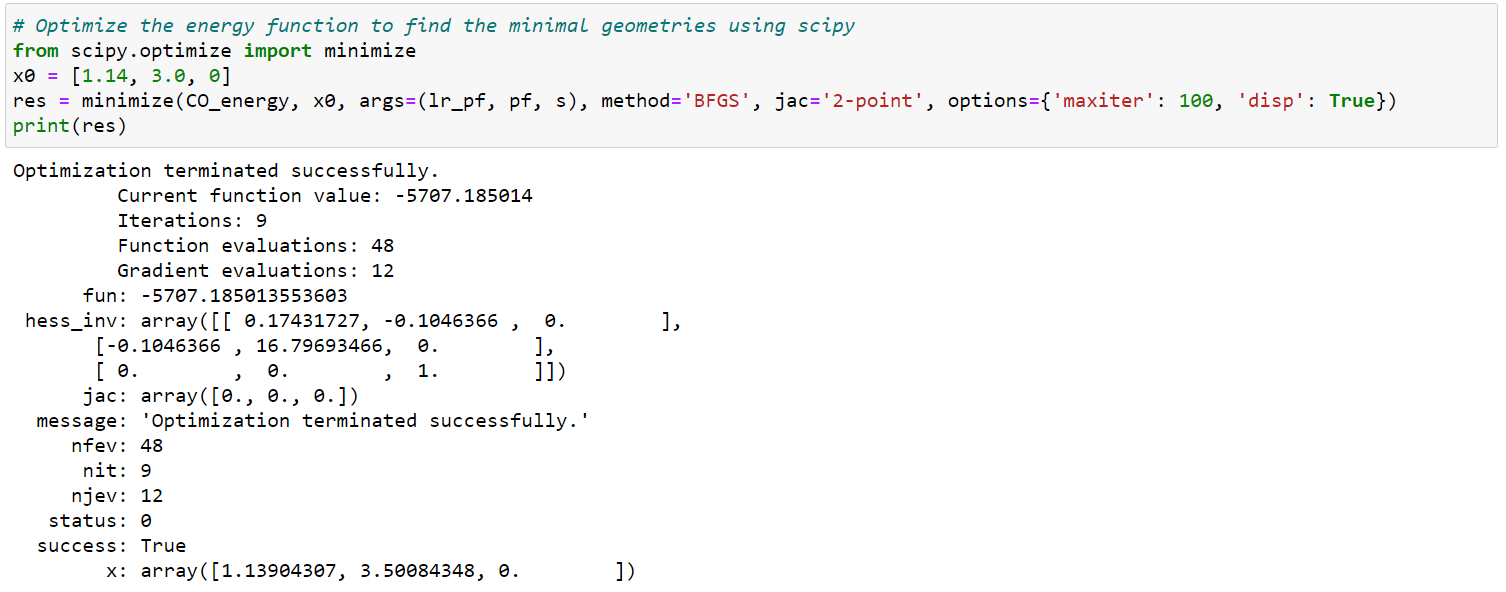
\includegraphics[scale=0.31]{opt.png}}
\caption{Minimize the CO energy to find the optimized geometry.}
\end{figure}

Here I use the polynomial regression model, optimize the parameters using BFGS algorithm and 2-point finite-difference gradient.
The initial guess is $r=1.14$, $R=3.0$, and $\theta = 0$.
I find one stable geometry at $r=1.139$, $R=3.501$, and $\theta = 0$, with energy $-5707.185014$.
This indicates a "C-down" geometry of the CO molecule, which is consistent with my chemistry knowledge.

\section{Summary and suggestions for next steps}\label{section-sugg}
In this report, I use the regression model to study the CO absorption on salt surface.
The 4th-order polynomial regression model successfully capture the relationship between CO geometry and its energy.
However, one fallacy I found is that the prediction will fail at geometries that is far away from the sampling area.
For example, the current data set only have data between $R=2.0$ and $R=5.0$. 
If I try $r=1.2$, $R=20.0$, and $\theta = 30$, the energy I got is $-4657.1123$, which is impossible since the CO energy should always been around $-5707.1$. 
To extend the usability, one solution is to collect more data beyond $R=2.0$ and $R=5.0$; the other solution is to integrate my domain knowledge: for R smaller than 2.0, the CO will be too close to the surface, the energy will be very high, while for R larger than 5.0, the energy should be almost unchanged since the interactions are negligible.
This mathematically implies an inverse exponential relationship between R and energy.
$$\delta E = Ce^{-\alpha R}$$
Therefore, one possible solution to try in the future is to conduct a logarithmic transformation for R before fitting.

%\bibliographystyle{alpha}
%\bibliography{references} % see references.bib for bibliography management

\end{document}
